\section{Deriving a pure functional approach}
\label{sec:functional_approach}

%2 main points from Henrik: 1.: try to stick to synchronous updates because this is how the real world works. 2.: get rid of globally shared mutable state as it complicates things extremely with reasoning
%clear conceptual formal model of what agents are and then structure my implementation around it

% TODO: put explanations before the code, otherwise readers get confused e.g. stepSimulation function

We presented a high-level agent-based approach to the SIR model in the previous section, which focused only on the states and the transitions, but we haven't talked about technical implementation details on how to actually implement such a state-machine. The authors of \cite{thaler_art_2017} discuss two fundamental problems of implementing an agent-based simulation from a programming language agnostic point of view. The first problem is how agents can be pro-active and the second how interactions and communication between agents can happen. For agents to be pro-active they must be able to perceive the passing of time, which means there must be a concept of an agent-process which executes over time. Interactions between agents can be reduced to the problem of how an agent can expose information about its internal state which can be perceived by other agents. \\
In this section we will derive a pure functional approach for an agent-based simulation of the SIR model in which we will pose solutions to the previously mentiond problems. We will start out with a very naive approach and show its limitations which we overcome by adding FRP. Then in further steps we will add more concepts and generalisations, ending up at the final approach which utilises monadic stream functions (MSF), a generalisation of FRP 
\footnote{The code of all steps can be accessed freely through the following URL: \url{https://github.com/thalerjonathan/phd/tree/master/public/purefunctionalepidemics/code}}.

% TODO: put all functions in italics

\subsection{Naive beginnings}
\label{sec:naive_beginnigs}
We start by modelling the states of the agents:

\begin{HaskellCode}
data SIRState = Susceptible | Infected TimeDelta | Recovered
\end{HaskellCode}

Agents are ill for some duration, meaning we need to keep track when a potentially infected agent recovers. Also a simulation is stepped in discrete or continuous time-steps thus we introduce a notion of \textit{time} and $\Delta t$ by defining:

\begin{HaskellCode}
type Time      = Double
type TimeDelta = Double
\end{HaskellCode}

Now we can represent every agent simply as the SIR state which includes its potential recovery time. We hold all our agents in a list:
\begin{HaskellCode}
type SIRAgent = SIRState
type Agents   = [SIRAgent]
\end{HaskellCode}

Next we need to think about how to actually step our simulation. For this we define a function which advances our simulation with a fixed $\Delta t$ until a given time $t$ where in each step the agents are processed and the output is fed back into the next step. This is the source of pro-activity as agents are executed in every time step and can thus initiate actions based on the passing of time.
As already mentioned, the agent-based implementation of the SIR model is inherently stochastic which means we need access to a random-number generator. We decided to use the Random Monad at this point as threading a generator through the simulation and the agents could become very cumbersome. Thus our simulation stepping runs in the Random Monad:
TODO: make clear we are stepping by a dt of 1.0 which is necessary below

\begin{HaskellCode}
runSimulation :: RandomGen g 
  => Time -> Agents -> Rand g [Agents]
runSimulation tEnd as = runSimulationAux 0 as []
  where
    runSimulationAux :: RandomGen g 
      => Time -> Agents -> [Agents] -> Rand g [Agents]
    runSimulationAux t as acc
      | t >= tEnd = return (reverse (as : acc))
      | otherwise = do
        as' <- stepSimulation as 
        runSimulationAux (t + 1.0) as' (as : acc)

stepSimulation :: RandomGen g => Agents -> Rand g Agents
stepSimulation as = mapM (runAgent as) as
\end{HaskellCode}

Now we can implement the behaviour of an individual agent. First we need to distinguish between the agents SIR states:

\begin{HaskellCode}
processAgent :: RandomGen g 
  => Agents -> SIRAgent -> Rand g SIRAgent
processAgent as Susceptible    = susceptibleAgent as
processAgent _  (Infected dur) = return (infectedAgent dur)
processAgent _  Recovered      = return Recovered
\end{HaskellCode}

An agent gets fed the states of all agents in the system from the previous time-step so it can draw random contacts - this is one, very naive way of implementing the interactions between agents.

From our implementation it becomes apparent that only the behaviour of a susceptible agent involves randomness and that a recovered agent is simply a sink - it does nothing and stays constant.

Lets look how we can implement the behaviour of a susceptible agent. It simply makes contact on average with a number of other agents and gets infected with a given probability if an agent it has contact with is infected.
When the agent gets infected, it calculates also its time of recovery by drawing a random number from the exponential distribution, meaning it is ill on average for \textit{illnessDuration}.
TODO: make clear that this only works for dt=1.0, if we change dt then we would need to adjust contact rate (multiply) but the discretisation using floor will lead to wrong results

\begin{HaskellCode}
susceptibleAgent :: RandomGen g => Agents -> Rand g SIRAgent
susceptibleAgent as = do
    -- draws from exponential distribution
    rc <- randomExpM (1 / contactRate) 
    cs <- replicateM (floor rc) (makeContact as)
    if or cs
      then infect
      else return Susceptible
  where
    makeContact :: RandomGen g => Agents -> Rand g Bool
    makeContact as = do
      randContact <- randomElem as
      case randContact of
        -- returns True with given probability 
        (Infected _) -> randomBoolM infectivity 
        _            -> return False

    infect :: RandomGen g => Rand g SIRAgent
    infect = randomExpM (1 / illnessDuration) 
               >>= \rd -> return (Infected rd)
\end{HaskellCode}

The infected agent is trivial. It simply recovers after the given illness duration which is implemented as follows:
TODO: explain that we are using fixed dt=1.0

\begin{HaskellCode}
infectedAgent :: TimeDelta -> TimeDelta -> SIRAgent
infectedAgent dur
    | dur' <= 0 = Recovered
    | otherwise = Infected dur'
  where
    dur' = dur - 1.0  
\end{HaskellCode}

\subsubsection{Results}
When running our naive implementation with a population size of 1,000 we get the dynamics as seen in Figure \ref{fig:sir_abs_dynamics_naive}. When comparing it to the dynamics of the analytical solution in Figure \ref{fig:sir_sd_dynamics}, the agent-based dynamics are not as smooth which stems from the fact that the agent-based approach is inherently discrete and stochastic \cite{macal_agent-based_2010}. Also we are using a $\Delta t = 1.0$ which means that we are under-sampling the contact-rate. We will will address this problem in the next section.

\begin{figure}
	\centering
	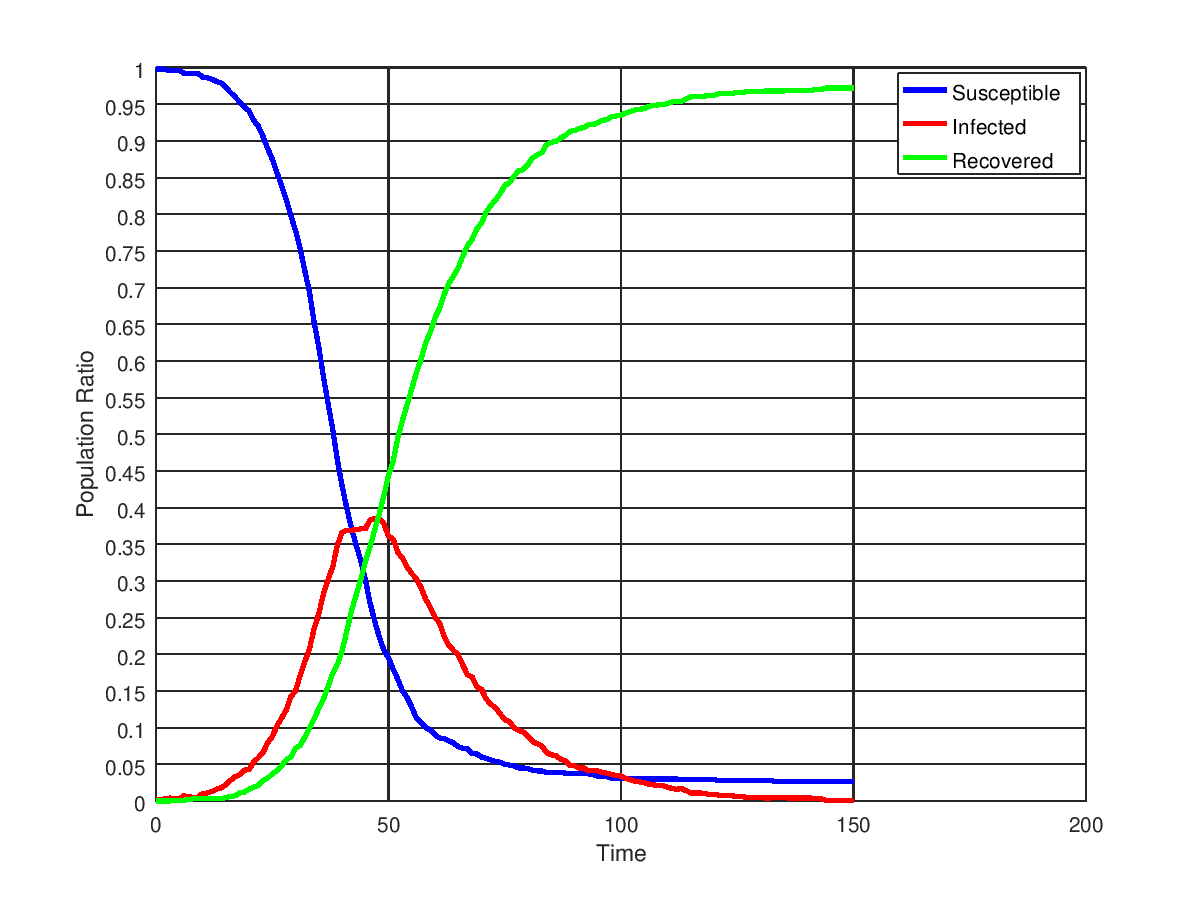
\includegraphics[width=0.35\textwidth, angle=0]{./fig/step1_randmonad/SIR_1000agents_150t_1dt.png}
	\caption{Naive simulation of SIR using the agent-based approach. Population of 1,000, contact rate $\beta = \frac{1}{5}$, infection probability $\gamma = 0.05$, illness duration $\delta = 15$ with initially 1 infected agent. Simulation run for 150 time-steps with fixed $\Delta t = 1.0$.}
	\label{fig:sir_abs_dynamics_naive}
\end{figure}

%\begin{figure}
%\begin{center}
%	\begin{tabular}{c}
%		\begin{subfigure}[b]{0.2\textwidth}
%			\centering
%			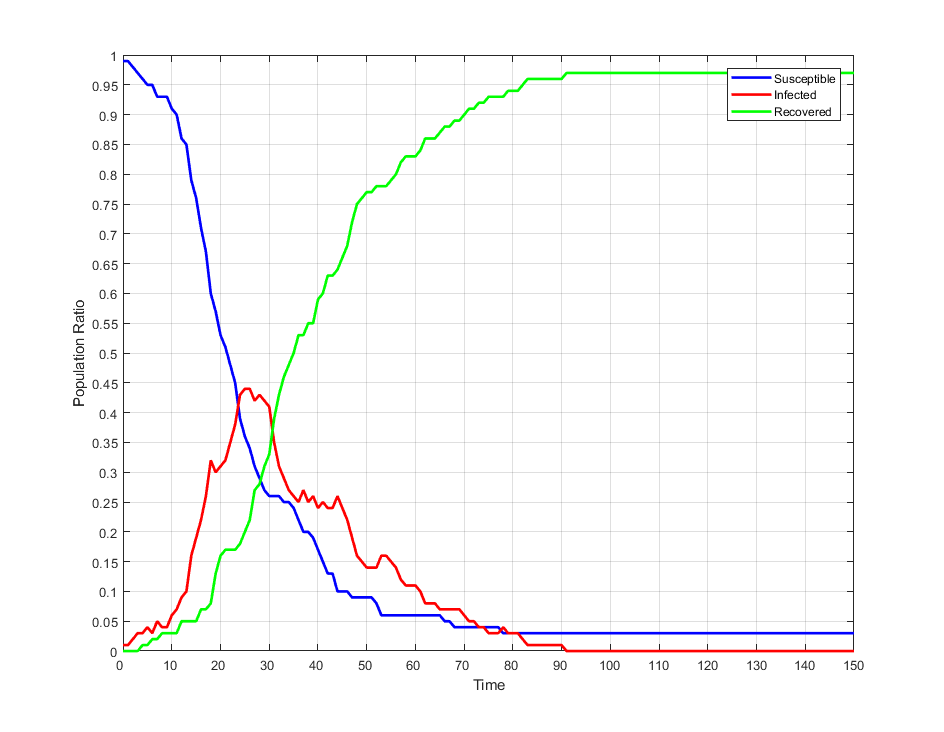
\includegraphics[width=1.0\textwidth, angle=0]{./fig/step1_randmonad/SIR_100agents_150t_1dt.png}
%			\caption{100 Agents}
%			\label{fig:sir_abs_approximating_1dt_100agents}
%		\end{subfigure}
    	
%    	&
%    	
%		\begin{subfigure}[b]{0.30\textwidth}
%			\centering
%			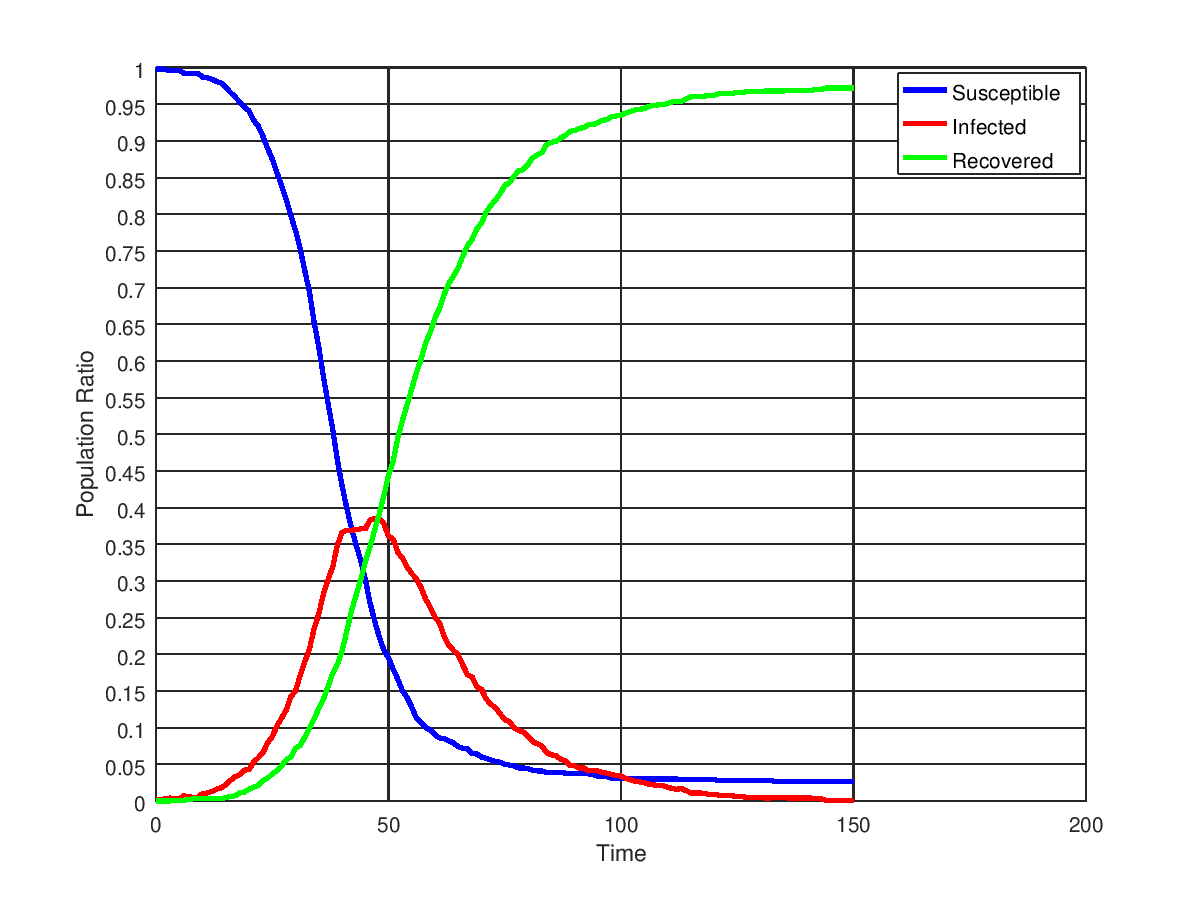
\includegraphics[width=1.0\textwidth, angle=0]{./fig/step1_randmonad/SIR_1000agents_150t_1dt.png}
%			\caption{1,000 Agents}
%			\label{fig:sir_abs_approximating_1dt_1000agents}
%		\end{subfigure}
%	\end{tabular}
%	\caption{TODO: use only 1000, a simulation with 100 has slightly different dynamics in SD as well! Naive simulation of SIR using the agent-based approach. Varying population size, contact rate $\beta = \frac{1}{5}$, infection probability $\gamma = 0.05$, illness duration $\delta = 15$ with initially 1 infected agent. Simulation run for 150 time-steps with fixed $\Delta t = 1.0$.} 
%	\label{fig:sir_abs_dynamics_naive}
%\end{center}
%\end{figure}

\subsubsection{Discussion}
Reflecting on our first naive approach we can conclude that it already introduced most of the fundamental concepts of ABS
\begin{itemize}
	\item Time - the simulation occurs over virtual time which is modelled explicitly divided into \textit{fixed} $\Delta t$ where at each step all agents are executed.
	\item Agents - we implement each agent as an individual, with the behaviour depending on its state.
	\item Feedback - the output state of the agent in the current time-step $t$ is the input state for the next time-step $t + \Delta t$.
	\item Environment - as environment we implicitly assume a fully-connected network (complete graph) where every agent 'knows' every other agent, including itself and thus can make contact with all of them.
	\item Stochasticity - it is an inherently stochastic simulation, which is indicated by the Random Monad type and the usage of \textit{randomBoolM} and \textit{randomExpM}.
	\item Deterministic - repeated runs with the same initial random-number generator result in same dynamics. This may not come as a surprise but in Haskell we can guarantee that property statically already at compile time because our simulation runs in the Random Monad and \textit{not} in the IO Monad. This guarantees that no external, uncontrollable sources of randomness can interfere with the simulation.
	\item Dynamics - with increasing number of agents the dynamics smooth out \cite{macal_agent-based_2010}.
\end{itemize}

TODO: problem is that we implicitly assume that TimeDelta is always 1.0, still it is not ensured in all agents

Nonetheless our approach has also weaknesses and dangers:
\begin{enumerate}
	\item We are implicitly assuming that our implementation is sampling with 1.0
	\item $\Delta t$ is passed explicitly as argument to the agent and needs to be dealt with explicitly. This is not very elegant and a potential source of errors - can we do better and find a more elegant solution? 
	\item The way our agents are represented is not very modular. The state of the agent is explicitly encoded in an ADT and when processing the agent, the behavioural function always needs to distinguish between the states. Can we express it in a more modular way e.g. continuations?
\end{enumerate}

We now move on to the next section in which we will address these points and the under-sampling issue.

\subsection{Functional Reactive Programming}
\label{sec:step2_frp}
As described in the Section \ref{sec:back_frp}, Arrowized FRP \cite{hughes_generalising_2000} is a way to implement systems  with continuous and discrete time-semantics where the central concept is the Signal Function, which can be understood as a process over time, mapping an input- to an output-signal. Technically speaking, a signal function is a continuation which allows to capture state using closures and hides away the $\Delta t$ which means that it is never exposed explicitly to the programmer, meaning it cannot be messed with.

The concept of processes over time is an ideal match for our agents and our system as a whole thus we will implement them and the whole system as signal functions.

\subsubsection{Implementation}
We start by defining the SIR states as ADTs and our agents as signal function (SF) which receives the SIR states of all agents as input and outputs the current SIR state of the agent:

\begin{HaskellCode}
data SIRState = Susceptible | Infected | Recovered

type SIRAgent = SF [SIRState] SIRState 
\end{HaskellCode}

Now we can define the behaviour of an agent to be the following:

\begin{HaskellCode}
sirAgent :: RandomGen g => g -> SIRState -> SIRAgent
sirAgent g Susceptible = susceptibleAgent g
sirAgent g Infected    = infectedAgent g
sirAgent _ Recovered   = recoveredAgent
\end{HaskellCode}

Depending on the initial state we return the corresponding behaviour. Note that we are passing a random-number generator instead of running in the Random Monad because signal functions as implemented in Yampa are not capable of being monadic. 

We see that the recovered agent ignores the random-number generator because a recovered agent does nothing, stays immune forever and can not get infected again in this model. Thus a recovered agent is a consuming state from which there is no escape, it simply acts as a sink which returns constantly \textit{Recovered}:

\begin{HaskellCode}
recoveredAgent :: SIRAgent
recoveredAgent = arr (const Recovered)
\end{HaskellCode}

Lets look how we can implement the behaviour of a susceptible agent. It makes contact \textit{on average} with $\beta$ other random agents. For every \textit{infected} agent it gets into contact with, it becomes infected with a probability of $\gamma$. If an infection happens, it makes the transition to the \textit{Infected} state. To make contact, it gets fed the states of all agents in the system from the previous time-step so it can draw random contacts - this is one, very naive way of implementing the interactions between agents.

Thus a susceptible agent behaves as susceptible until it becomes infected. Upon infection an \textit{Event} is returned which results in switching into the \textit{infectedAgent} SF, which causes the agent to behave as an infected agent from that moment on. When an infection event occurs we change the behaviour of an agent using the Yampa combinator \textit{switch}, which is quite elegant and expressive as it makes the change of behaviour at the occurrence of an event explicit. Note that to make contact \textit{on average}, we use Yampas \textit{occasionally} function which requires us to carefully select the right $\Delta t$ for sampling the system as will be shown in results. 

%\begin{samepage}
\begin{HaskellCode}
susceptibleAgent :: RandomGen g => g -> SIRAgent
susceptibleAgent g = 
    switch (susceptible g) (const (infectedAgent g))
  where
    susceptible :: RandomGen g 
      => g -> SF [SIRState] (SIRState, Event ())
    susceptible g = proc as -> do
      makeContact <- occasionally g (1 / contactRate) () -< ()
      if isEvent makeContact
        then (do
          -- draw random element from the list
          a <- drawRandomElemSF g -< as
          case a of
            Infected -> do
              -- returns True with given probability
              i <- randomBoolSF g infectivity -< ()
              if i
                then returnA -< (Infected, Event ())
                else returnA -< (Susceptible, NoEvent)
             _       -> returnA -< (Susceptible, NoEvent))
        else returnA -< (Susceptible, NoEvent)
\end{HaskellCode}
%\end{samepage}

To deal with randomness in an FRP way we implemented additional signal functions built on the \textit{noiseR} function provided by Yampa. This is an example for the stream character and statefulness of a signal function as it allows to keep track of the changed random-number generator internally through the use of continuations and closures. Here we provide the implementation of \textit{randomBoolSF}. \textit{drawRandomElemSF} works similar but takes a list as input and returns a randomly chosen element from it:

\begin{HaskellCode}
randomBoolSF :: RandomGen g => g -> Double -> SF () Bool
randomBoolSF g p = proc _ -> do
  r <- noiseR ((0, 1) :: (Double, Double)) g -< ()
  returnA -< (r <= p)
\end{HaskellCode}

An infected agent recovers \textit{on average} after $\delta$ time units. This is implemented by drawing the duration from an exponential distribution \cite{borshchev_system_2004} with $\lambda = \frac{1}{\delta}$ and making the transition to the \textit{Recovered} state after this duration. Thus the infected agent behaves as infected until it recovers, on average after the illness duration, after which it behaves as a recovered agent by switching into \textit{recoveredAgent}. As in the case of the susceptible agent, we use the \textit{occasionally} function to generate the event when the agent recovers. Note that the infected agent ignores the states of the other agents as its behaviour is completely independent of them.

\begin{HaskellCode}
infectedAgent :: RandomGen g => g -> SIRAgent
infectedAgent g = switch infected (const recoveredAgent)
  where
    infected :: SF [SIRState] (SIRState, Event ())
    infected = proc _ -> do
      recEvt <- occasionally g illnessDuration () -< ()
      let a = event Infected (const Recovered) recEvt
      returnA -< (a, recEvt)
\end{HaskellCode}

For running the simulation we use Yampas function \textit{embed}:

\begin{HaskellCode}
runSimulation :: RandomGen g 
  => g -> Time -> DTime -> [SIRState] -> [[SIRState]]
runSimulation g t dt as 
    = embed (stepSimulation sfs as) ((), dts)
  where
    steps     = floor (t / dt)
    dts       = replicate steps (dt, Nothing)
    n         = length as
    (rngs, _) = rngSplits g n [] -- unique rngs for each agent
    sfs       = zipWith sirAgent rngs as
\end{HaskellCode}

What we need to implement next is a closed feedback-loop - the heart of every agent-based simulation. Fortunately, \cite{nilsson_functional_2002, courtney_yampa_2003} discusses implementing this in Yampa. The function \textit{stepSimulation} is an implementation of such a closed feedback-loop. It takes the current signal functions and states of all agents, runs them all in parallel and returns this step's new agent states. Note the use of \textit{notYet} which is required because in Yampa switching occurs immediately at $t = 0$. If we don't delay the switching at $t = 0$ until the next step, we would enter an infinite switching loop - \textit{notYet} simply delays the first switching until the next time-step.

\begin{HaskellCode}
stepSimulation :: [SIRAgent] -> [SIRState] -> SF () [SIRState]
stepSimulation sfs as =
    dpSwitch
      -- feeding the agent states to each SF
      (\_ sfs' -> (map (\sf -> (as, sf)) sfs'))
      -- the signal functions
      sfs
      -- switching event, ignored at t = 0         
      (switchingEvt >>> notYet)
      -- recursively switch back into stepSimulation         
      stepSimulation                            
  where
    switchingEvt :: SF ((), [SIRState]) (Event [SIRState])
    switchingEvt = arr (\ (_, newAs) -> Event newAs)
\end{HaskellCode}

Yampa provides the \textit{dpSwitch} combinator for running signal functions in parallel, which has the following type-signature:

\begin{HaskellCode}
dpSwitch :: Functor col
         -- routing function
         => (forall sf. a -> col sf -> col (b, sf))
         -- SF collection
         -> col (SF b c)
         -- SF generating switching event     
         -> SF (a, col c) (Event d)
         -- continuation to invoke upon event           
         -> (col (SF b c) -> d -> SF a (col c))
         -> SF a (col c)
\end{HaskellCode}

Its first argument is the pairing-function which pairs up the input to the signal functions - it has to preserve the structure of the signal function collection. The second argument is the collection of signal functions to run. The third argument is a signal function generating the switching event. The last argument is a function which generates the continuation after the switching event has occurred. \textit{dpSwitch} returns a new signal function which runs all the signal functions in parallel and switches into the continuation when the switching event occurs. The d in \textit{dpSwitch} stands for decoupled which guarantees that it delays the switching until the next time-step: the function into which we switch is only applied in the next step, which prevents an infinite loop if we switch into a recursive continuation.

Conceptually, \textit{dpSwitch} allows us to recursively switch back into the \textit{stepSimulation} with the continuations and new states of all the agents after they were run in parallel. 

\subsubsection{Results}
The dynamics generated by this step can be seen in Figure \ref{fig:sir_abs_dynamics_frp}. 

\begin{figure}
\begin{center}
	\begin{tabular}{c c}
		\begin{subfigure}[b]{0.22\textwidth}
			\centering
			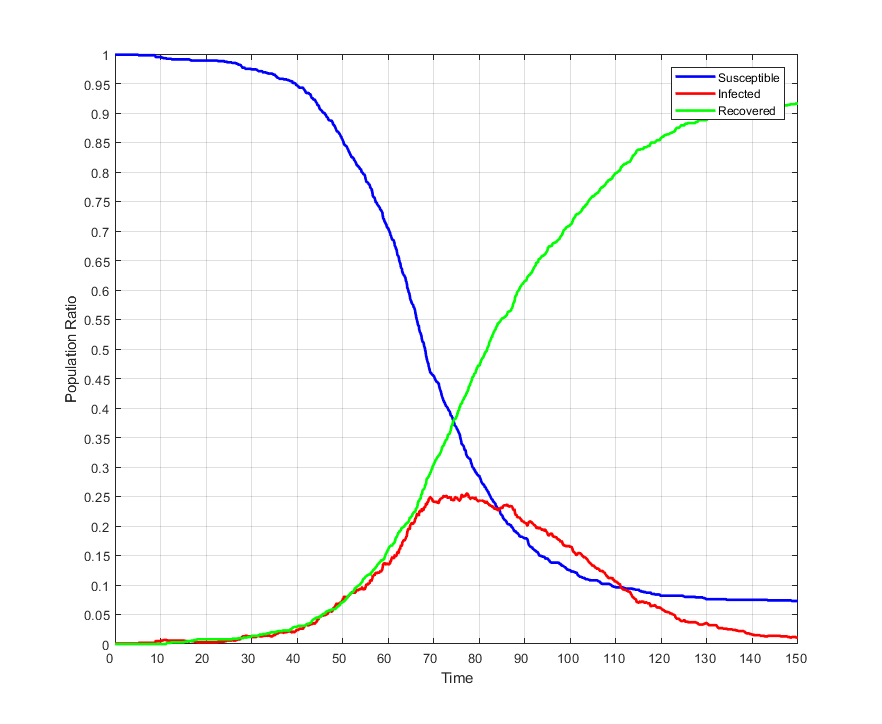
\includegraphics[width=1\textwidth, angle=0]{./fig/step2_yampa/SIR_1000agents_150t_01dt.png}
			\caption{$\Delta t = 0.1$}
			\label{fig:sir_abs_approximating_01dt_1000agents}
		\end{subfigure}
		
		&
    	
		\begin{subfigure}[b]{0.22\textwidth}
			\centering
			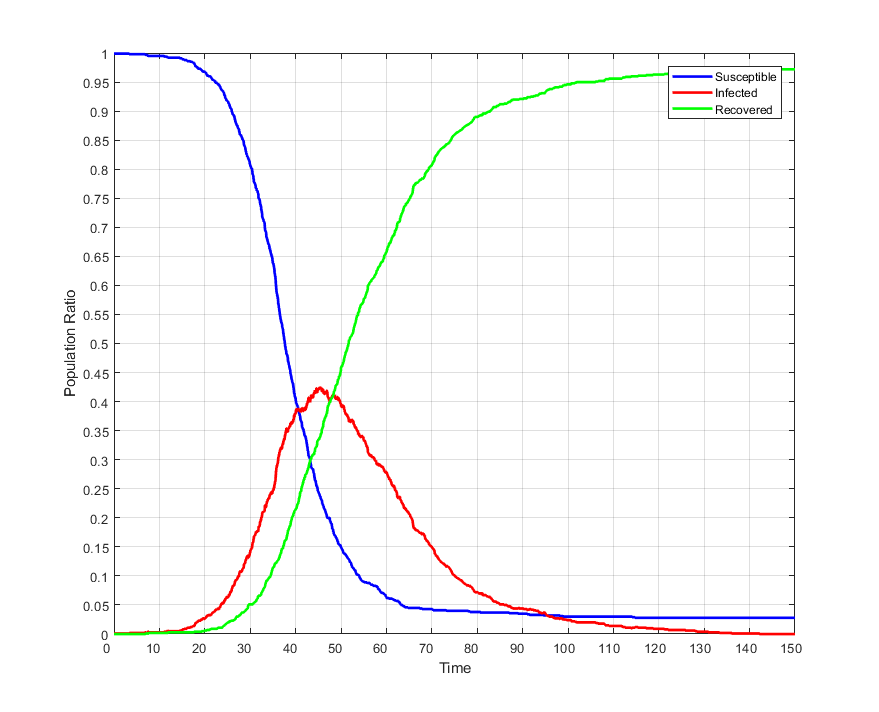
\includegraphics[width=1\textwidth, angle=0]{./fig/step2_yampa/SIR_1000agents_150t_001dt.png}
			\caption{$\Delta t = 0.01$}
			\label{fig:sir_abs_approximating_001dt_1000agents}
		\end{subfigure}
	\end{tabular}
	
	\caption{FRP simulation of agent-based SIR showing the influence of different $\Delta t$. Population size of 1,000 with contact rate $\beta = \frac{1}{5}$, infection probability $\gamma = 0.05$, illness duration $\delta = 15$ with initially 1 infected agent. Simulation run for 150 time-steps with respective $\Delta t$.} 
	\label{fig:sir_abs_dynamics_frp}
\end{center}
\end{figure}

By following the FRP approach we assume a continuous flow of time which means that we need to select a \textit{correct} $\Delta t$ otherwise we would end up with wrong dynamics. The selection of a correct $\Delta t$ depends in our case on \textit{occasionally} in the \textit{susceptible} behaviour, which randomly generates an event on average with \textit{contact rate} following the exponential distribution. To arrive at the correct dynamics, this requires us to sample \textit{occasionally}, and thus the whole system, with small enough $\Delta t$ which matches the frequency of events generated by \textit{contact rate}. If we choose a too large $\Delta t$, we loose events which will result in wrong dynamics as can be seen in Figure \ref{fig:sir_abs_approximating_01dt_1000agents}. This issue is known as under-sampling and is described in Figure \ref{fig:sampling_issue}.

\begin{figure}
\begin{center}
	\begin{tabular}{c}
		\begin{subfigure}[b]{0.3\textwidth}
			\centering
			
\includegraphics[width=1\textwidth, angle=0]{./fig/diagrams/Undersampling.png}
			\caption{Under-sampling}
			\label{fig:undersampling}
		\end{subfigure}
		
		\\
		
		\begin{subfigure}[b]{0.3\textwidth}
			\centering
			
\includegraphics[width=1\textwidth, angle=0]{./fig/diagrams/Supersampling.png}
			\caption{Super-sampling}
			\label{fig:supersampling}
		\end{subfigure}
	\end{tabular}
	
	\caption{A visual explanation of under-sampling and super-sampling. The black dots represent the time-steps of the simulation. The red dots represent virtual events which occur at specific points in continuous time. In the case of under-sampling, 3 events occur in between the two time steps but \textit{occasionally} only captures the first one. By increasing the sampling frequency either through a smaller $\Delta t$ or super-sampling all 3 events can be captured.} 
	\label{fig:sampling_issue}
\end{center}
\end{figure}

For tackling this issue we have two options. The first one is to use a smaller $\Delta t$ as can be seen \ref{fig:sir_abs_approximating_001dt_1000agents}, which results in the whole system being sampled more often, thus reducing performance. The other option is to implement super-sampling and apply it to \textit{occasionally} which would allow us to run the whole simulation with $\Delta t = 1.0$ and only sample the \textit{occasionally} function with a much higher frequency.

An approach to super-sampling would be to introduce a new combinator to Yampa which allows us to super-sample other signal functions. 

\begin{HaskellCode}
superSampling :: Int -> SF a b -> SF a [b]
\end{HaskellCode}

It evaluates the \textit{SF} argument for \textit{n} times, each with $\Delta t = \frac{\Delta t}{n}$ and the same input argument \textit{a} for all \textit{n} evaluations. At time 0 no super-sampling is performed and just a single output of the \textit{SF} argument is calculated. A list of \textit{b} is returned with length of \textit{n} containing the result of the \textit{n} evaluations of the \textit{SF} argument. If 0 or less super samples are requested exactly one is calculated. We could then wrap the occasionally function which would then generate a list of events. We have investigated super-sampling more in-depth but have to omit this due to lack of space.

\subsubsection{Discussion}
We can conclude that our first step already introduced most of the fundamental concepts of ABS:
\begin{itemize}
	\item Time - the simulation occurs over virtual time which is modelled explicitly divided into \textit{fixed} $\Delta t$ where at each step all agents are executed.
	\item Agents - we implement each agent as an individual, with the behaviour depending on its state.
	\item Feedback - the output state of the agent in the current time-step $t$ is the input state for the next time-step $t + \Delta t$.
	\item Environment - as environment we implicitly assume a fully-connected network (complete graph) where every agent 'knows' every other agent, including itself and thus can make contact with all of them.
	\item Stochasticity - it is an inherently stochastic simulation, which is indicated by the random-number generator and the usage of \textit{occasionally}, \textit{randomBoolSF} and \textit{drawRandomElemSF}.
	\item Deterministic - repeated runs with the same initial random-number generator result in same dynamics. This may not come as a surprise but in Haskell we can guarantee that property statically already at compile time because our simulation runs \textit{not} in the IO Monad. This guarantees that no external, uncontrollable sources of non-determinism can interfere with the simulation.
\end{itemize}

Using FRP in the instance of Yampa results in clarity, expressivity and robustness of our implementation. State is implicitly encoded, depending on which signal function is active. By using explicit time-semantics with \textit{occasionally} we can achieve extremely fine grained stochastics by sampling the system with small $\Delta t$: we are treating it as a truly continuous time-driven agent-based system.

A very severe problem, very hard to find with testing but detectable with in-depth validation analysis, is the fact that in the \textit{susceptible} agent the same random-number generator is used in \textit{occasionally}, \textit{drawRandomElemSF} and \textit{randomBoolSF}. This means that all three stochastic functions, which should be independent from each other, are inherently correlated. This is something one wants to prevent under all circumstances in a simulation, as it can invalidate the dynamics on a very subtle level, and indeed we have tested the influence of the correlation in this example and it has an impact. We left this severe bug in for explanatory reasons, as it shows an example where functional programming actually encourages very subtle bugs if one is not careful. A possible solution would be to simply split the initial random-number generator in \textit{sirAgent} three times (using one of the splited generators for the next split) and pass three random-number generators to \textit{susceptible}.

So far we have an acceptable implementation of an agent-based SIR approach. What we are lacking at the moment is a general treatment of an environment. To conveniently introduce it we want to make use of monads which is not possible using Yampa. In the next step we make the transition to Monadic Stream Functions as introduced in Dunai \cite{perez_functional_2016} which allows FRP within a monadic context.

\begin{comment}
\subsection{Adding arbitrary data-flow}
\label{sec:step3_dataflow}
As already mentioned previously, by revealing the state of every agent to all other agents makes the interactions implicit and deprives the agent of its control over which internal state it wants to reveal to the other agents. As a remedy we introduce data-flows which allow an agent to send arbitrary data to other agents which makes the communication and feedback amongst agents explicit. We cannot express this directly with Yampa combinators as data-flow in Yampa is hard-wired at compile-time so we need to implement our own mechanism because agent interaction is random. The data will be collected from the sending agents and distributed to the receivers after each step, which means that we have a delay of one $\Delta t$ and a round-trip takes $2 \Delta t$ - which is exactly the feedback behaviour we had before.
This change requires a different approach of how the agents interact with each other: a susceptible agent then sends to a random agent a data-flow indicating a contact. Only infected agents need to reply to such contact requests by revealing that they are infected. The susceptible agents then need to check for incoming replies which means they were in contact with an infected agent.
The deeper motivation behind this data-flow mechanism is the need of an ABS to provide some means to allow agents to interact and communicate with each other. In object-oriented approaches this is rather trivial because agents can call methods of other agents directly and implicitly mutate the other agents state. When following a \textit{pure} approach in Haskell this becomes much more difficult and the data-flow mechanism is our ad-hoc solution for this problem.

\subsubsection{Implementation}
First we need a way of addressing agents, which we do by introducing unique agent ids. Also we need a data-package which identifies the receiver and carries the data:
\begin{HaskellCode}
type AgentId     = Int
type DataFlow d = (AgentId, d)
\end{HaskellCode}

Next we need more general input and output types of our agents signal functions. We introduce a new input type which holds both the agent id of the agent and the incoming data-flows from other agents:

\begin{HaskellCode}
data AgentIn d = AgentIn
  { aiId   :: AgentId
  , aiData :: [DataFlow d] } 
\end{HaskellCode}

We also introduce a new output type which holds both the outgoing data-flows to other agents and the observable state the agent wants to reveal to the outside world:

\begin{HaskellCode}
data AgentOut o d = AgentOut
  { aoData        :: [DataFlow d]
  , aoObservable  :: o }
\end{HaskellCode}

Note that by making the observable state explicit in the types we give the agent further control of what it can reveal to the outside world which allows an even stronger separation between the agents internal state and what the agent wants the world to see.

Now we can then generalise the agents signal function to the following type:
\begin{HaskellCode}
type Agent o d = SF (AgentIn d) (AgentOut o d)
\end{HaskellCode}

For our SIR implementation we need concrete types, so we need to define what the type parameters \textit{o} and \textit{d} are. For \textit{d} we use an ADT as contact-message. As type of the observable state we use the existing SIR state. Now we can define the type synonyms for our SIR implementation:
\begin{HaskellCode}
data SIRMsg      = Contact SIRState deriving Eq
type SIRAgentIn  = AgentIn SIRMsg
type SIRAgentOut = AgentOut SIRState SIRMsg
type SIRAgent    = Agent SIRState SIRMsg
\end{HaskellCode}

Next we are going to re-implement the agent-behaviour:

\begin{HaskellCode}
sirAgent :: RandomGen g => g -> [AgentId] -> SIRState -> SIRAgent
sirAgent g ais Susceptible = susceptibleAgent g ais
sirAgent g _   Infected    = infectedAgent g
sirAgent _ _   Recovered   = recoveredAgent
\end{HaskellCode}

The initial behaviour is the same as previously but it now takes a list of agent ids as additional parameter. With data-flow we need to know the ids of the agents we are communicating with - we need to know our neighbourhood, or seen differently: we need to have access to the environment we are situated in. In our case our environment is a fully connected read-only network in which all agents know all other agents. The easiest way of representing a fully connected network (complete graph) is simply using a list. 
The implementation of the recovered agent is still the same, its just a sink which ignores the environment and the random-number generator. 

\begin{HaskellCode}
recoveredAgent :: SIRAgent
recoveredAgent = arr (const (agentOut Recovered))
\end{HaskellCode}

Note that instead of returning just a SIR state now the output of an agents signal function is of type \textit{AgentOut}:

\begin{HaskellCode}
agentOut :: o -> AgentOut o d
agentOut o = AgentOut {
    aoData       = []
  , aoObservable = o }
\end{HaskellCode}

The behaviour of the infected agent now explicitly ignores the environment which was not apparent previously on this level:

\begin{HaskellCode}
infectedAgent :: RandomGen g => g -> SIRAgent
infectedAgent g = switch infected (const recoveredAgent)
  where
    infected :: SF SIRAgentIn (SIRAgentOut, Event ())
    infected = proc ain -> do
      recEvt <- occasionally g illnessDuration () -< ()
      let a  = event Infected (const Recovered) recEvt
          ao = respondToContactWith Infected ain (agentOut a)
      returnA -< (ao, recEvt)
\end{HaskellCode}

The implementation of the infected agent is essentially the same as previously but it now needs to reply to incoming contact data-flows with an "Infected" reply. This makes the difference to the previous step very explicit: in the data-flow approach agents now make explicit contact with each other which means that the susceptible agent sends out contact data-flows to which only infected agents need to reply. Note that at the moment of recovery the agent can still infect others because it will still reply with Infected. The response mechanism is implemented in \textit{respondToContactWith}:

\begin{HaskellCode}
respondToContactWith :: SIRState -> SIRAgentIn -> SIRAgentOut -> SIRAgentOut
respondToContactWith state = onData respondToContactWithAux
  where
    respondToContactWithAux :: DataFlow SIRMsg -> SIRAgentOut -> SIRAgentOut
    respondToContactWithAux (senderId, Contact _) = dataFlow (senderId, Contact state)
    
onData :: (DataFlow d -> acc -> acc) -> AgentIn d -> acc -> acc
onData df ai a = foldr df a (aiData ai)

dataFlow :: DataFlow d -> AgentOut o d -> AgentOut o d
dataFlow df ao = ao { aoData = df : aoData ao }
\end{HaskellCode}

Note that the order of data-packages in a data-flow is not specified and must not matter as it happens virtually at the same time, thus we always append at the front of the outgoing data-flow list.

Lets look at the susceptible agent behaviour. Again the implementation is very similar to the previous step with the fundamental difference being how contacts are made and how infections occur. First the agent checks if it got infected. This happens if an infected agent replies to the susceptible agents contact \textit{and} the susceptible agent got infected with the given probability. Note that \textit{gotInfected} runs in the Random Monad which we run using \textit{runRand} and the random-number generator. To update our random-number generator to the changed one, we use the \textit{rec} keyword of the Arrow notation \cite{paterson_new_2001}, which allows us to refer to a variable before it is defined. In combination with \textit{iPre} we introduced a local state - the random-number generator - which changes in every step. The function \textit{iPre :: a -> SF a a} delays the input by one time-step, returns it in the next time-step and is initialized with an initial value. If the agent got infected, it simply returns an AgentOut with Infected as observable state and a switching event which indicates the switch to infected behaviour.
If the agent is not infected it draws from \textit{occasionally} to determine if it should make contact with a random agent. In case it should make contact it simply sends a data-package with the contact susceptible data to the receiver - note that only an infected agent will reply.

\begin{HaskellCode}
susceptibleAgent :: RandomGen g => g -> [AgentId] -> SIRAgent
susceptibleAgent g ais = switch (susceptible g) (const (infectedAgent g))
  where
    susceptible :: RandomGen g => g -> SF SIRAgentIn (SIRAgentOut, Event ())
    susceptible g0 = proc ain -> do
      rec
        g <- iPre g0 -< g'
        let (infected, g') = runRand (gotInfected infectivity ain) g

      if infected 
        then returnA -< (agentOut Infected, Event ())
        else (do
          makeContact <- occasionally g (1 / contactRate) () -< ()
          contactId   <- drawRandomElemSF g                  -< ais
          let ao = agentOut Susceptible
          if isEvent makeContact
            then returnA -< (dataFlow (contactId, Contact Susceptible) ao, NoEvent)
            else returnA -< (ao, NoEvent))
            
gotInfected :: RandomGen g => Double -> SIRAgentIn -> Rand g Bool
gotInfected p ain = onDataM gotInfectedAux ain False
  where
    gotInfectedAux :: RandomGen g => Bool -> DataFlow SIRMsg -> Rand g Bool
    gotInfectedAux False (_, Contact Infected) = randomBoolM p
    gotInfectedAux x _ = return x
    
onDataM :: Monad m => (acc -> DataFlow d -> m acc) -> AgentIn d -> acc -> m acc
onDataM df ai acc = foldM df acc (aiData ai)
\end{HaskellCode}

Stepping the simulation now works a little bit different as the input/output types have changed and we need to collect and distribute the data-flow amongst the agents:

\begin{HaskellCode}
stepSimulation :: [SIRAgent] -> [SIRAgentIn] -> SF () [SIRAgentOut]
stepSimulation sfs ains =
    dpSwitch
      (\_ sfs' -> (zip ains sfs')) -- pairing up the AgentIn to the corresponding SF
      sfs                          -- the signal functions
      (switchingEvt >>> notYet)    -- switching event, ignored at t = 0
      stepSimulation               -- recursively switch back into stepSimulation
  where
    switchingEvt :: SF ((), [SIRAgentOut]) (Event [SIRAgentIn])
    switchingEvt = proc (_, aos) -> do
      let ais      = map aiId ains       -- collect all AgentIds
          aios     = zip ais aos         -- pair up AgentIns with their AgentOuts
          nextAins = distributeData aios -- distribute the data-flows to receivers
      returnA -< Event nextAins
\end{HaskellCode}

The distribution of the data-flows happens in the \textit{distributeData} function of \textit{switchingEvt} and is then passed on to the continuation-generation function as previously. Note that due to lack of space we can't give an implementation of \textit{distributeData} but we provide the type.

\begin{HaskellCode}
distributeData :: [(AgentId, AgentOut o d)] -> [AgentIn d]
\end{HaskellCode}

\subsubsection{Discussion}
It seems that by introducing the data-flow mechanism we have increased complexity but we have gained a lot as well. Data-flows make the feedback between agents explicit and give the agents full control over the data which is revealed to other agents. This also makes the fact even more explicit, that we cannot fix the connections between the agents already at compile time e.g. by connecting SFs which is done in many Yampa applications \cite{nilsson_functional_2002}, \cite{courtney_yampa_2003}, \cite{nilsson_declarative_2014} because agents interact with each other randomly. One can look at the data-flow mechanism as a kind of messaging but there are fundamental differences. Messaging almost always comes up as an approach to managing concurrency and involves stateful message-boxes which can be checked an emptied by the receivers - this is not the case with the data-flow mechanism which behaves indeed as a flow where data is not stored in a message box but is only present in the current simulation-step and if ignored by the agent, it will be gone in the next step.
Also by distinguishing between the internal and the observable state of the agent, we give the agent even more control of what is visible to the outside world.
So far we have an acceptable implementation of an agent-based SIR approach. The next steps focus on introducing more concepts and generalising our implementation so far. What we are lacking at the moment is a general treatment of an environment. To conveniently introduce it we want to make use of monads which is not possible using Yampa. In the next step we make the transition to Monadic Stream Functions (MSF) as introduced in Dunai \cite{perez_functional_2016} which allows to do FRP within a monadic context.
\end{comment}

\subsection{Generalising to Monadic Stream Functions}
\label{sec:generalising_msfs}
A part of the library Dunai is BearRiver, a wrapper which re-implements Yampa on top of Dunai, which should allow us to easily replace Yampa with MSFs. This will enable us to run arbitrary monadic computations in a signal function, solving our problem of correlated random numbers through the use of the Random Monad.

\subsubsection{Identity Monad}
We start by making the transition to BearRiver by simply replacing Yampas signal function by BearRivers', which is the same but takes an additional type parameter \textit{m}, indicating the monadic context. If we replace this type-parameter with the Identity Monad, we should be able to keep the code exactly the same, because BearRiver re-implements all necessary functions we are using from Yampa. We simply re-define the agent signal function, introducing the monad stack our SIR implementation runs in:

\begin{HaskellCode}
type SIRMonad = Identity
type SIRAgent = SF SIRMonad [SIRState] SIRState
\end{HaskellCode}

\subsubsection{Random Monad}
Using the Identity Monad does not gain us anything but it is a first step towards a more general solution. Our next step is to replace the Identity Monad by the Random Monad, which will allow us to run the whole simulation within the Random Monad with the full features of FRP, finally solving the problem of correlated random numbers in an elegant way. We start by re-defining the SIRMonad and SIRAgent:

\begin{HaskellCode}
type SIRMonad g = Rand g
type SIRAgent g = SF (SIRMonad g) [SIRState] SIRState
\end{HaskellCode}

The question is now how to access this Random Monad functionality within the MSF context. For the function \textit{occasionally}, there exists a monadic pendant \textit{occasionallyM} which requires a MonadRandom type-class. Because we are now running within a MonadRandom instance we simply replace \textit{occasionally} with \textit{occasionallyM}. 

\begin{HaskellCode}
occasionallyM :: MonadRandom m => Time -> b -> SF m a (Event b)
-- can be used through the use of arrM and lift
randomBoolM :: RandomGen g => Double -> Rand g Bool
-- this can be used directly as a SF with the arrow notation
drawRandomElemSF :: MonadRandom m => SF m [a] a
\end{HaskellCode}

\subsubsection{Discussion} 
Running in the Random Monad solved the problem of correlated random numbers and elegantly guarantees us that we won't have correlated stochastics as discussed in the previous section. In the next step we introduce the concept of an explicit discrete 2D environment.

\subsection{Adding an environment}
\label{sec:adding_env}
So far we have implicitly assumed a fully connected network amongst agents, where each agent can see and 'knows' every other agent. This is a valid environment and in accordance with the System Dynamics inspired implementation of the SIR model but does not show the real advantage of ABS to situate agents within arbitrary environments. Often, agents are situated within a discrete 2D environment \cite{epstein_growing_1996} which is simply a finite $N x M$ grid with either a Moore or von Neumann neighbourhood (Figure \ref{fig:abs_neighbourhoods}). Agents are either static or can move freely around with cells allowing either single or multiple occupants.

We can directly map the SIR model to a discrete 2D environment by placing the agents on a corresponding 2D grid with an unrestricted neighbourhood. The behaviour of the agents is the same but they select their interactions directly from the shared read-only environment, which will be passed to the agents as input. This allows agents to read the states of all their neighbours which tells them if a neighbour is infected or not. To show the benefit over the System Dynamics approach  and for purposes of a more interesting approach, we restrict the neighbourhood to Moore (Figure \ref{fig:moore_neighbourhood}).

\begin{figure}
\begin{center}
	\begin{tabular}{c c}
		\begin{subfigure}[b]{0.2\textwidth}
			\centering
			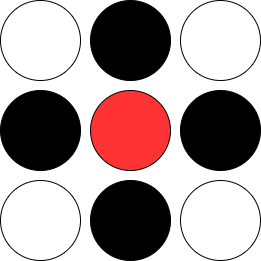
\includegraphics[width=0.5\textwidth, angle=0]{./fig/diagrams/neumann.png}
			\caption{von Neumann}
			\label{fig:neumann_neighbourhood}
		\end{subfigure}
    	&
		\begin{subfigure}[b]{0.2\textwidth}
			\centering
			
\includegraphics[width=0.5\textwidth, angle=0]{./fig/diagrams/moore.png}
			\caption{Moore}
			\label{fig:moore_neighbourhood}
		\end{subfigure}
    \end{tabular}
	\caption{Common neighbourhoods in discrete 2D environments of Agent-Based Simulation.}
	\label{fig:abs_neighbourhoods}
\end{center}
\end{figure}

We also implemented this spatial approach in Java using the well known ABS library RePast \cite{north_complex_2013}, to have a comparison with a state of the art approach and came to the same results as shown in Figure \ref{fig:sir_dunai}. This supports, that our pure functional approach can produce such results as well and compares positively to the state of the art in the ABS field.

\subsubsection{Implementation}
We start by defining the discrete 2D environment for which we use an indexed two dimensional array. Each cell stores the agent state of the last time-step, thus we use the \textit{SIRState} as type for our array data. Also, we re-define the agent signal function to take the structured environment \textit{SIREnv} as input instead of the list of all agents as in our previous approach. As output we keep the \textit{SIRState}, which is the state the agent is currently in. Also we run in the Random Monad as introduced before to avoid the random number correlation. 

\begin{HaskellCode}
type Disc2dCoord = (Int, Int)
type SIREnv      = Array Disc2dCoord SIRState

type SIRAgent g  = SF (Rand g) SIREnv SIRState
\end{HaskellCode}

Note that the environment is not returned as output because the agents do not directly manipulate the environment but only read from it. Again, this enforces the semantics of the \textit{parallel} update-strategy through the types where the agents can only see the previous state of the environment and see the actions of other agents reflected in the environment only in the next step.

Note that we could have chosen to use a StateT transformer with the \textit{SIREnv} as state, instead of passing it as input, with the agents then able to arbitrarily read/write, but this would have violated the semantics of our model because actions of agents would have become visible within the same time-step.

The implementation of the susceptible, infected and recovered agents are almost the same with only the neighbour querying now slightly different. 

Stepping the simulation needs a new approach because in each step we need to collect the agent outputs and update the environment for the next next step. For this we implemented a separate MSF, which receives the coordinates for every agent to be able to update the state in the environment after the agent was run. Note that we need use \textit{mapM} to run the agents because we are running now in the context of the Random Monad. This has the consequence that the agents are in fact run sequentially one after the other but because they cannot see the other agents actions nor observe changes in the shared read-only environment, it is \textit{conceptually} a \textit{parallel} update-strategy where agents run in lock-step, isolated from each other at conceptually the same time.
  
\begin{HaskellCode}
simulationStep :: RandomGen g => [(SIRAgent g, Disc2dCoord)]
               -> SIREnv -> SF (Rand g) () SIREnv
simulationStep sfsCoords env = MSF (\_ -> do
  let (sfs, coords) = unzip sfsCoords 
  -- run agents sequentially but with shared, read-only environment
  ret <- mapM (`unMSF` env) sfs
  -- construct new environment from all agent outputs for next step
  let (as, sfs') = unzip ret
      env' = foldr (\ (a, coord) envAcc -> updateCell coord a envAcc) 
               env (zip as coords)

      sfsCoords' = zip sfs' coords
      cont       = simulationStep sfsCoords' env'
  return (env', cont))
 
updateCell :: Disc2dCoord -> SIRState -> SIREnv -> SIREnv
\end{HaskellCode}

\subsubsection{Results}
We implemented rendering of the environments using the gloss library which allows us to cycle arbitrarily through the steps and inspect the spreading of the disease over time visually as seen in Figure \ref{fig:sir_dunai}.

\begin{figure}
\begin{center}
	\begin{tabular}{c c}
		\begin{subfigure}[b]{0.2\textwidth}
			\centering
			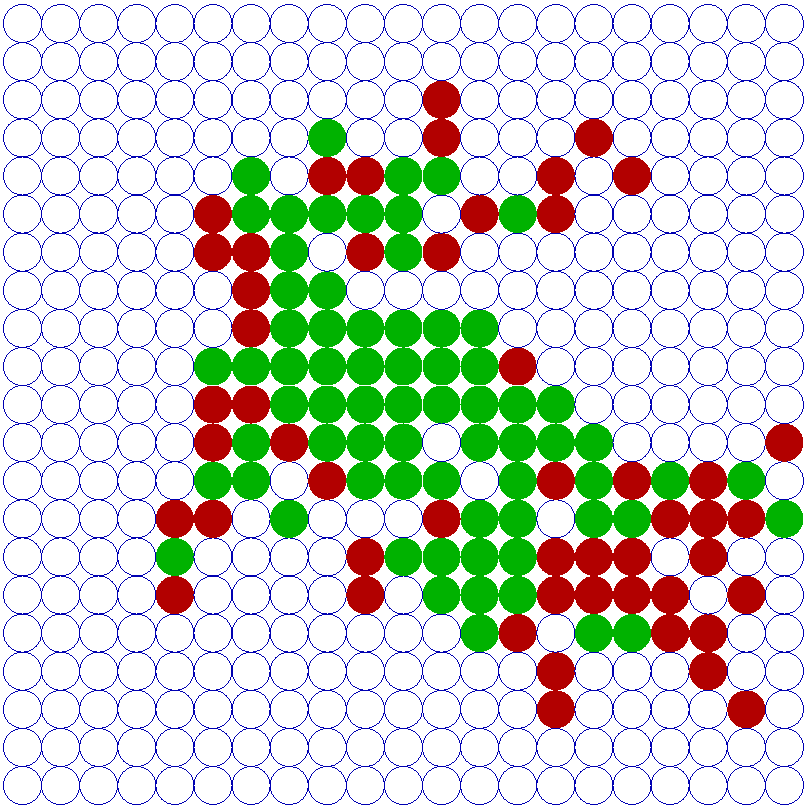
\includegraphics[width=1\textwidth, angle=0]{./fig/SIR_Dunai/SIR_Dunai_dt001_environment.png}
			\caption{Environment at $t = 50$}
			\label{fig:sir_dunai_env}
		\end{subfigure}
    	
    	&
  
		\begin{subfigure}[b]{0.23\textwidth}
			\centering
			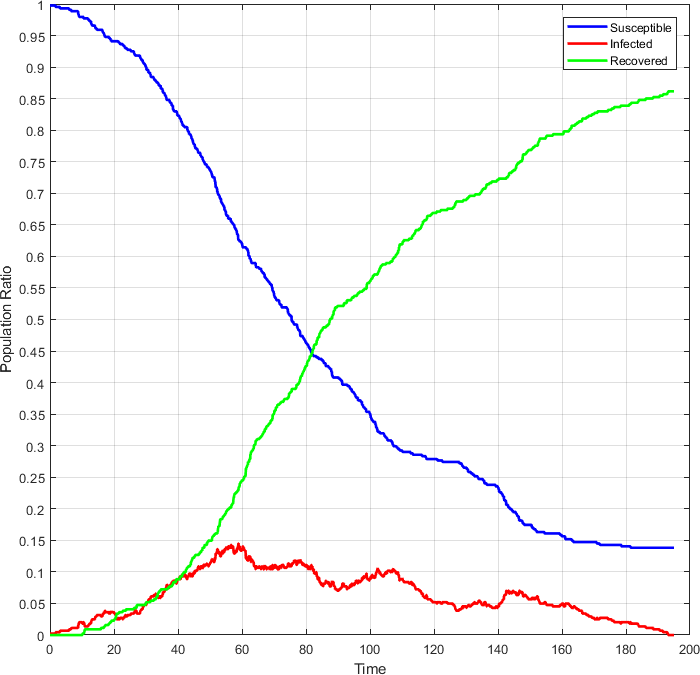
\includegraphics[width=1\textwidth, angle=0]{./fig/SIR_Dunai/SIR_Dunai_dt001.png}
			\caption{Dynamics over time}
			\label{fig:sir_dunai_env_dynamics}
		\end{subfigure}
	\end{tabular}
	
	\caption{Simulating the agent-based SIR model on a 21x21 2D grid with Moore neighbourhood (Figure \ref{fig:moore_neighbourhood}), a single infected agent at the center and same SIR parameters as in Figure \ref{fig:sir_sd_dynamics}. Simulation run until $t = 200$ with fixed $\Delta t = 0.01$. Last infected agent recovers around $t = 194$. The susceptible agents are rendered as blue hollow circles for better contrast.}
	\label{fig:sir_dunai}
\end{center}
\end{figure}

Note that the dynamics of the spatial SIR simulation which are seen in Figure \ref{fig:sir_dunai_env_dynamics} look quite different from the reference dynamics of Figure \ref{fig:sir_sd_dynamics}. This is due to a much more restricted neighbourhood which results in far fewer infected agents at a time and a lower number of recovered agents at the end of the epidemic, meaning that fewer agents got infected overall.

\subsubsection{Discussion}
By introducing a structured environment with a Moore neighbourhood, we showed the ABS ability to place the heterogeneous agents in a generic environment, which is the fundamental advantage of an agent-based approach over other simulation methodologies and allows us to simulate much more realistic scenarios.

Note, that an environment is not restricted to be a discrete 2D grid and can be anything from a continuous N-dimensional space to a complex network - one only needs to change the type of the environment and agent input and provide corresponding neighbourhood querying functions. 

% this is omited for now as it takes too much time and involves too many details but would need much more explanation still
%\section{Agent transactions}
Imagine two agents A and B want to engage in a bartering process where agent A, is the seller who wants to sell an asset to agent B who is the buyer. Agent A sends Agent B a sell offer depending on how much agent A values this asset. Agent B receives this sell offer, checks if the price satisfies its utility, if it has enough wealth to buy the asset and replies with either a refusal or its own price offer. Agent A then considers agent Bs offer and if it is happy it replies to agent B with an acceptance of the offer, removes the asset from its inventory and increases its wealth. Agent B receives this acceptance offer, puts the asset in its inventory and decreases its wealth (note that this process could involve a potentially arbitrary number of steps without loss of generality).
We can see this behaviour as a kind of multi-step transactional behaviour because agents have to respect their budget constraints which means that they cannot spend more wealth or assets than they have. This implies that they have to 'lock' the asset and the amount of cash they are bartering about during the bartering process. If both come to an agreement they will swap the asset and the cash and if they refuse their offers they have to 'unlock' them.
In classic OO implementations it is quite easy to implement this as normally only one agent is active at a time due to sequential (discrete event scheduling approach) scheduling of the simulation. This allows then agent A which is active, to directly interact with agent B through method calls. The sequential updating ensures that no other agent will touch the asset or cash and the direct method calls ensure a synchronous updating of the mutable state of both objects with no time passing between these updates.

\subsection{Implementation}
We start with the implementation of step 4 with the Random Monad and remove the data-flows from AgentIn and AgentOut. We then add a field in AgentOut which allows the agent to indicate that it wants to start a transaction with another agent with an initial data-package. Also we add a field in AgentIn which indicates an incoming transaction request from another agent with the given data-package. In addition we need another field in AgentOut which allows the agent to indicate that it accepts the incoming request:

\begin{HaskellCode}
data AgentIn d = AgentIn
  { aiId        :: !AgentId
  , aiRequestTx :: !(Event (AgentData d))}

data AgentOut m o d = AgentOut
  { aoObservable :: !o
  , aoRequestTx  :: !(Event (AgentData d, AgentTX m o d))
  , aoAcceptTx   :: !(Event (d, AgentTX m o d))}
\end{HaskellCode}

We run the transactions in the specialised agent-transaction signal-functions \textit{AgentTX} with different input and output types. This allows us to restrict the possible actions of an agent within a transaction:

\begin{HaskellCode}
type AgentTX m o d = SF m (AgentTXIn d) (AgentTXOut m o d)
\end{HaskellCode}

The input \textit{AgentTXIn} to an agent-transaction holds optional data and flags which indicate that the other agent has either committed or aborted the transaction.

\begin{HaskellCode}
data AgentTXIn d = AgentTXIn
  { aiTxData   :: Maybe d
  , aiTxCommit :: Bool
  , aiTxAbort  :: Bool
  }
\end{HaskellCode}

The output \textit{AgentTXOut} of an agent-transaction hold optional data a flag to abort the transaction and optional commit data which is Just in case the agent wants to commit. When committing the agent has to provide a potentially changed AgentOut and optionally a new agent behaviour signal-function. If the agent provides a signal-function when committing, the behaviour of the agent after the transaction will be this signal-function. If no signal-function is provided then the original one will be used.

\begin{HaskellCode}
data AgentTXOut m o d = AgentTXOut
  { aoTxData   :: Maybe d
  , aoTxCommit :: Maybe (AgentOut m o d, Maybe (Agent m o d))
  , aoTxAbort  :: Bool
  }
\end{HaskellCode}

We also provide type aliases for our SIR implementation:
\begin{HaskellCode}
type SIRMonad g    = Rand g
data SIRMsg        = Contact SIRState deriving (Show, Eq)
type SIRAgentIn    = AgentIn SIRMsg
type SIRAgentOut g = AgentOut (SIRMonad g) SIRState SIRMsg
type SIRAgent g    = Agent (SIRMonad g) SIRState SIRMsg
type SIRAgentTX g  = AgentTX (SIRMonad g) SIRState SIRMsg
\end{HaskellCode}

Stepping the simulation is now slightly more complex as in every step we need to run the transactions. Fortunately it is easy to provide customised implementations of MSFs in dunai, which is a bit more tricky in Yampa and requires to expose internals.

\begin{HaskellCode}
stepSimulation :: RandomGen g => [SIRAgent g] -> [SIRAgentIn] -> SF (SIRMonad g) () [SIRAgentOut g]
stepSimulation sfs ains = MSF (\_ -> do
  res <- mapM (\ (ai, sf) -> unMSF sf ai) (zip ains sfs)
  let aos  = fmap fst res
      sfs' = fmap snd res
      ais  = map aiId ains
      aios = zip ais aos

  -- this works only because runTransactions is stateless and runs the SFs with dt = 0
  ((aios', sfs''), _) <- unMSF runTransactions (aios, sfs')

  let aos'  = map snd aios'
      ains' = map agentIn ais
      ct    = stepSimulation sfs'' ains'
      
  return (aos', ct))
\end{HaskellCode}

The implementation of \textit{runTransactions} is quite involved and omitted here because it would require too much space, but we will give a short informal description. All agents are iterated in an unspecified sequence and if an agent requests a transaction the other agent is looked up and the transaction-pair is run. This is done recursively until there are no transaction requests any-more (note that through the AgentOut of a committed transaction, an agent can request a new transaction within the same time-step). Running a transaction-pair works as follows:
The target agents signal-function is run again (resulting in a second, or third,... execution, depending on how many transactions have this agent as target) but now with a $\Delta t = 0$. The target agent can then accept the incoming transaction or simply ignore it. If it is ignored the transaction will never start. The fact that the target agent signal-function is run more than once within a simulation step but with a $\Delta t = 0$ requires agents to make their actions time-dependent \textit{but} they must listen to incoming transactions independent of time. The implementation of the infected agent below will make this more clear.
When the transaction is accepted the system switches to running the transaction signal-functions after another with passing the data forward and backward between the two agents. It is most important to note that again the signal functions are run with $\Delta t = 0$ because conceptionally transactions happen \textit{instantaneously} without time advancing. This has important implications, and means that we cannot use any time-accumulating function e.g. integral or after within a transaction - simply because it makes no sense as no time passes. If \textit{both} agents commit the transaction their new AgentOuts will replace the ones for the current simulation-step. If either one agent aborts the transaction the current AgentOuts of the current simulation-step will be used.

We provide a sequence diagram of data-flow in a multi-step negotiation as described in the introduction for a visual explanation of the complex protocol which is going on in a transaction.

Now it is time to look at the new agent implementations which use now the agent-transaction mechanism. The recovered agent is exactly the same but the susceptible and infected agent behaviour are very different now. Lets first look at the susceptible agent:

\begin{HaskellCode}
susceptibleAgent :: RandomGen g => [AgentId] -> SIRAgent g
susceptibleAgent ais = proc _ -> do
    makeContact <- occasionallyM (1 / contactRate) () -< ()

    if not (isEvent makeContact)
      then returnA -< agentOut Susceptible
      else (do
        contactId <- drawRandomElemS -< ais
        returnA -< requestTx 
                    (contactId, Contact Susceptible) 
                    susceptibleTx
                    (agentOut Susceptible))
  where
    susceptibleTx :: RandomGen g => SIRAgentTX g
    susceptibleTx = proc txIn ->
      -- should have always tx data
      if hasTxDataIn txIn 
          then (do
            let (Contact s) = txDataIn txIn 
            -- only infected agents reply, but make it explicit
            if Infected /= s
              -- don't commit with continuation, no change in behaviour
              then returnA -< commitTx (agentOut Susceptible) agentTXOut
              else (do
                infected <- arrM_ (lift (randomBoolM infectivity)) -< ()
                if infected
                  -- commit with continuation as we switch into infected behaviour
                  then returnA -< commitTxWithCont 
                                    (agentOut Infected) 
                                    infectedAgent
                                    agentTXOut
                  -- don't commit with continuation, no change in behaviour
                  else returnA -< commitTx (agentOut Susceptible) agentTXOut))
          else returnA -< abortTx agentTXOut
\end{HaskellCode}

Instead of using a switch the susceptible agent behaves completely time-dependent and occasionally starts a new agent-transaction with a random agent. The function \textit{susceptibleTx} handles the reply of the other agent. Note that we only commit with a continuation in case the agent becomes infected.

The infected agent is slightly less complex and still uses the switch mechanism:
\begin{HaskellCode}
infectedAgent :: RandomGen g => SIRAgent g
infectedAgent = switch infected (const recoveredAgent)
  where
    infected :: RandomGen g => SF (SIRMonad g) SIRAgentIn (SIRAgentOut g, Event ())
    infected = proc ain -> do
      recEvt <- occasionallyM illnessDuration () -< ()
      let a = event Infected (const Recovered) recEvt
      -- note that at the moment of recovery the agent can still infect others
      -- because it will still reply with Infected
      let ao = agentOut a

      if isRequestTx ain 
        then (returnA -< (acceptTX 
                           (Contact Infected)
                           (infectedTx ao)
                           ao, recEvt))
        else returnA -< (ao, recEvt)

    infectedTx :: RandomGen g => SIRAgentOut g -> SIRAgentTX g
    infectedTx ao = proc _ ->
      -- it is important not to commit with continuation as it
      -- would reset the time of the SF to 0. Still occasionally
      -- would work as it does not accumulate time but functions
      -- like after or integral would fail
      returnA -< commitTx ao agentTXOut
\end{HaskellCode}

The agent acts time-dependent which in this case is the transition from infected to recovered - if occasionallyM is run with $\Delta t = 0$ then no Event can happen. The agent checks on every function call of infected for incoming transactions and accepts them all, independent of the state - only susceptible agents request transactions anyway. The agent simply replies with a Contact Infected and immediately commits the transaction in the transaction signal-function but does not switch into a new continuation.

\subsection{Discussion}
Note that the transactions run in the same monad as the normal agent behaviour signal-function which allows to add an environment as in step 5. In this case care must be taken when one has changed the environment but aborts the transaction as a roll back of the environment won't happen automatically. A different approach would allow to run the TX in a different monad and bring in e.g. the  transactional state monad Control.Monad.Tx which supports rolling back of changes to the state.

The concept of agent-transactions is not explicitly known in the agent-based community and a novel development of this paper. The reason for this is that agent-transactions are already implicitly available in traditional OO implementations in which agents can call each others methods and change their state. By implementing this necessary and important concept in a pure functional approach we arrived at agent-transactions which make these synchronous, instantaneous, one-to-one interactions explicit.\\

% we have also a step7: event-driven implemented but omit it due to lack of space

\begin{comment}
\subsection{Further Steps}
\subsubsection{Agent-Transactions}
Agent-transactions are necessary when an arbitrary number of interactions between two agents need to happen instantaneously without time-lag. The use-case for this are price negotiations between multiple agents where each pair of agents needs to come to an agreement in the same time-step \cite{epstein_growing_1996}. In object-oriented programming, the concept of synchronous communication between agents is implemented directly with method calls. We have implemented synchronous interactions, which we termed agent-transactions in an additional step which we had to omit due to lack of space. We solved it pure functionally by running the signal functions of the transacting agent pair as often as their protocol requires but with $\Delta t=0$, which indicates the instantaneous character of agent-transactions.

\subsubsection{Event Scheduling}
Our approach is inherently time-driven where the system is sampled with fixed $\Delta t$. The other fundamental way to implement an ABS in general, is to follow an event-driven approach \cite{meyer_event-driven_2014} which is based on the theory of discrete-event simulation \cite{zeigler_theory_2000}. In such an approach the system is not sampled in fixed $\Delta t$ but advanced as events occur where the system stays constant in between. Depending on the model, in an event-driven approach it may be more natural to express the requirements of the model. In an additional step we have implemented a rudimentary event-driven approach which allows the scheduling of events but had to omit it due to lack of space. Using the flexibility of MSFs we added a State transformer to the monad stack which allows enqueuing of events into a priority queue. The simulation is advanced by processing the next event at the top of the queue which means running the MSF of the agent which receives the event. The simulation terminates if there are either no more events in the queue or after a given number of events or if the simulation time has advanced to some limit. Having made the transition to MSFs, implementing this feature was quite easy which shows the power and strength of the generalised approach to FRP using MSFs.

\subsubsection{Dynamic Agent creation}
In the SIR model, the agent population stays constant - agents don't die and no agents are created during simulation - but some simulations \cite{epstein_growing_1996} require dynamic agent creation and destruction. We can easily add and remove agents signal functions in the recursive switch after each time-step. The only problem is that creating new agents requires unique agent ids but with the transition to MSFs we can add a monadic context which allows agents to draw the next unique agent id when they create a new agent. %The id generation process should happen in the agent as the creating agent almost always needs then to communicate with this new agent. If we defer the id generation to the simulation system itself then we need a mechanism to feed it back to the creating agent, which could become quite cumbersome.
\end{comment}